\chapter{Usability - Tests}
\begin{tiny}
	RS, TF\\
	\ \\
\end{tiny}
Um das \textbf{ofCourse} System bezüglich dem Gesichtspunkt der Benutzbarkeit bzw. der Benutzerfreundlichkeit zu testen,
wurden unvoreingenommene Testpersonen gesucht, welche das System testeten und anschließend das System, aufgrund der
während der Tests gewonnenen Eindrücke evaluierten.\\
\\
Die Usability - Test wurden durchgeführt um die Erfüllung des Punktes {\it Benutzbarkeit} der Qualitätsbestimmungen
aus dem Pflichtenheft, welcher von uns als sehr wichtig eingestuft wurde, zu validieren.

\section{Durchführung}
Für die Durchführung der Test wurden zufällig ausgewählte Personen vom Campus herangezogen. Einziger Gesichtspunkt für die Auswahl der Testpersonen war, dass sie das System ofCourse bisher nicht kannten und auch noch nie damit gearbeitet haben und somit unvoreingenommen an die Test herangingen.\ \\
\ \\
Wenn die angesprochene Person sich für den Test bereit erklärt hatte, wurde sie von uns zufällig einer der Testgruppen zugeordnet und über den Ablauf des Tests aufgeklärt. Die Testpersonen erhielten je nach Gruppe ihre Arbeitsanweisungen und wurden belehrt, dass sie den Test eigenständig und wenn möglich ohne Unterbrechung durchführen sollten. Anschließend sollten die Testpersonen eigenständig die Arbeitsanweisungen ausführen. Fragen der Probanden bezüglich den Aufgaben wurden seitens der Testleiter im Normalfall nicht beantwortet.\\
\ \\
Nach Abschluss des Test wurden die Testpersonen dazu aufgefordert den Feedback - Fragebogen \ref{fig:OfCourseFeedback} auszufüllen.\\
Die Testleiter notierten bei jeder Person die Dauer, welche für die Bearbeitung der Aufgaben benötigt wurde.



\section{Material}
Für die Durchführung der Tests wurden folgende Materialien angefertigt.
\subsection{Testanweisungen}
Für die Durchführung der Test wurden Arbeitsanweisungen für die Testpersonen erstellt. Zum einen mit dem Zweck den Test in einem angemessenen zeitlichen Rahmen durchführbar zu machen, zum anderen um die Vergleichbarkeit der verschiedenen Testdurchläufe zu ermöglichen.\ \\
Es wurden drei verschiedene Arbeitsanweisungen erstellt, nämlich für Testgruppe 1, Testgruppe 2, Testgruppe 3. Die Arbeitsanweisungen\ref{fig:Anweisungen1} der Testgruppe 1 beinhalten Funktionen, welche einem {\it registrierten Benutzer} zur Verfügung stehen und umfassten unter anderem das Registrieren im System und das Anmelden zu einem Kurs.\\
Die Arbeitsanweisungen\ref{fig:Anweisungen2} der Gruppe 2  beinhalten Funktionen von {\it Kursleitern}, beispielsweise das Bearbeiten eines Kurses bzw. das Anlegen von Kurseinheiten.\\
Die Anweisungen\ref{fig:Anweisungen3} für Testgruppe 3 beinhalten schließlich Funktionen, welche nur dem {\it Administrator} zur Verfügung stehen, wie etwa das Festlegen des Überziehungskredits oder das Erstellen eines Kurses.
\subsection{Fragebogen}
Um die Eindrücke der Testpersonen festzuhalten, wurde ein kurzer Fragebogen erstellt. Dieser ist zweigeteilt. \\
Der erste Teil besteht aus fünf kurzen Aussagen, welche die Testpersonen auf einer Skala von {\it Trifft gar nicht zu} bis 
{\it Trifft voll zu} bewerten sollen. Diese Aussagen beziehen sich auf verschiedene Aspekte der Benutzbarkeit.
Zu diesen zählen unter anderem die Gestaltung der Oberfläche, die intuitive Bedienbarkeit und das schnelle Auffinden der Funktionen.\\
(vgl. Feedback - Fragebogen ofCourse \ref{fig:OfCourseFeedback} ).\ \\
\ \\
Der zweite Teil des Fragebogens besteht aus offenen Fragen, welche von den Testpersonen kurz zu beantworten sind.\\
Unter anderem wird dabei gefragt, welcher Aspekt des Systems den Benutzer besonders gut gefallen hat und welche Verbesserungen er sich am System wünschen würde.\\
Zum Schluss des Fragebogens können die Testpersonen unter dem Punkt {\it Meine letzten Worte...} noch einen allgemeinen Kommentar zum System abgeben. \\
(vgl. Feedback - Fragebogen ofCourse \ref{fig:OfCourseFeedback} ).\ \\


\section{Ergebnisse}
Um die Eindrücke der Testpersonen protokollieren und auswerten zu können, wurden sie gebeten einen Fragebogen auszufüllen.
Im folgenden werden die gewonnenen Ergebnisse anhand der einzelnen Punkte des Fragebogens aufgeführt. Zusätzlich
wurde auch noch die Bearbeitungszeit der Test erhoben.

\subsection{Frage 1}
\begin{center}
	{\it Ich habe mich in ofCourse schnell zurechtgefunden.}
\end{center}
\begin{figure}[h]
\centering
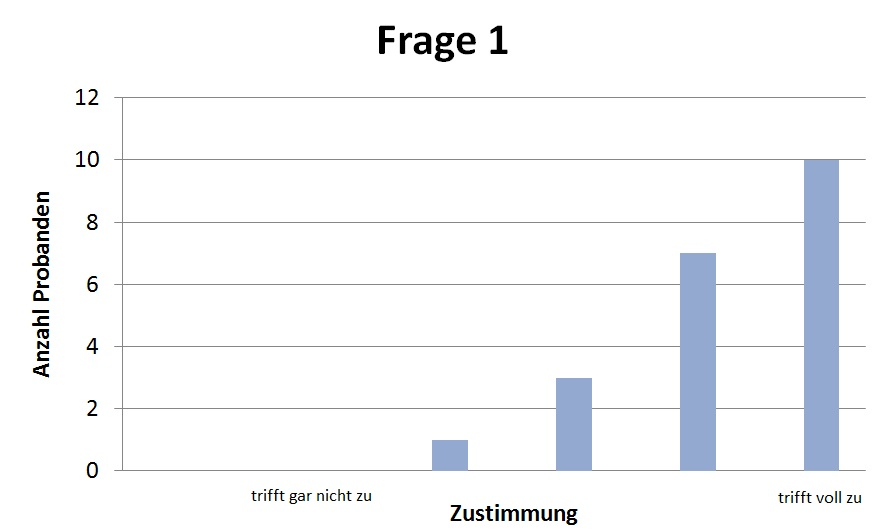
\includegraphics[width=0.7\linewidth]{img/Frage1}
\caption{Gesamtergebnis Frage 1}
\label{fig:Frage1}
\end{figure}

\subsection{Frage 2}
\begin{center}
	{\it ofCourse ist übersichtlich und leicht verständlich.}
\end{center}
\begin{figure}[h]
\centering
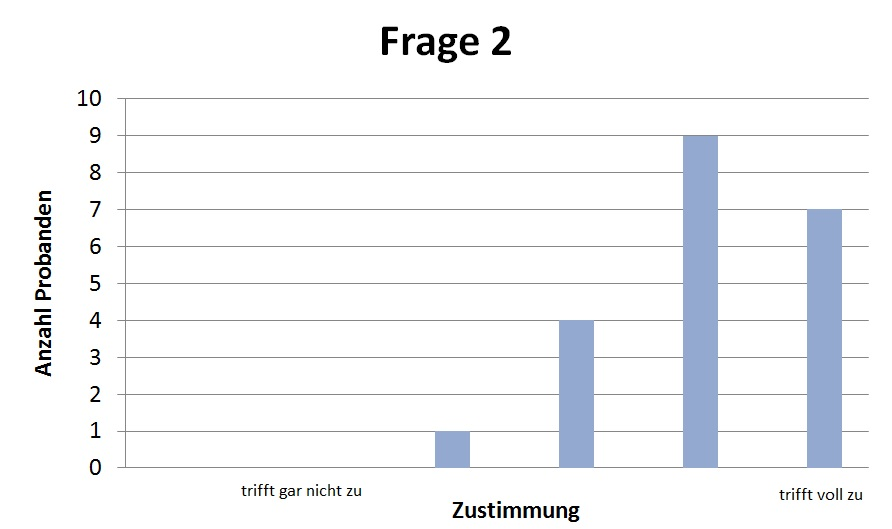
\includegraphics[width=0.7\linewidth]{img/Frage2}
\caption{Gesamtergebnis Frage 2}
\label{fig:Frage2}
\end{figure}


\subsection{Frage 3}
\begin{center}
	{\it Die gestellten Aufgaben waren mit ofCourse einfach zu lösen.}
\end{center}
\begin{figure}[h]
\centering
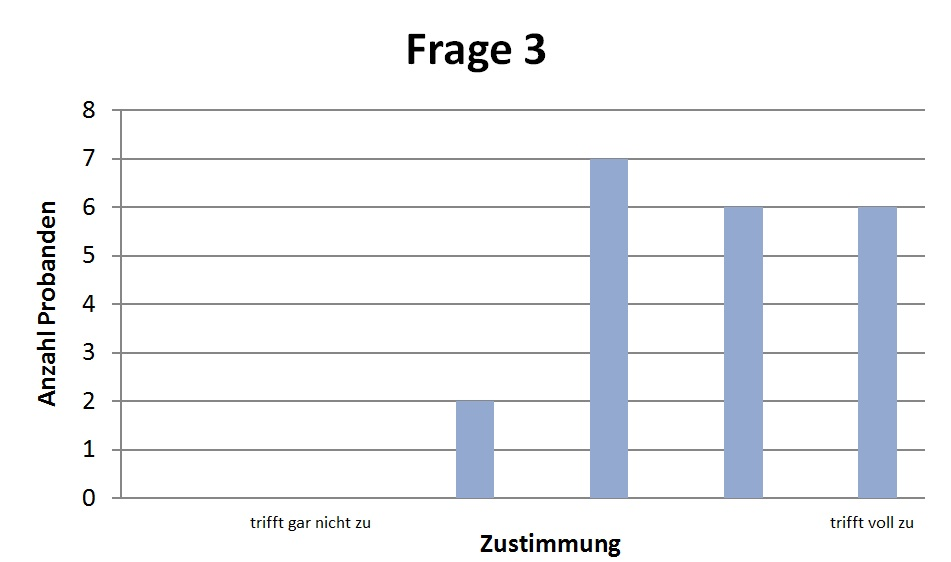
\includegraphics[width=0.7\linewidth]{img/Frage3}
\caption{Gesamtergebnis Frage 3}
\label{fig:Frage3}
\end{figure}

\subsection{Frage 4}
\begin{center}
	{\it Das Design von ofCourse spricht mich an.}
\end{center}
\begin{figure}[h]
\centering
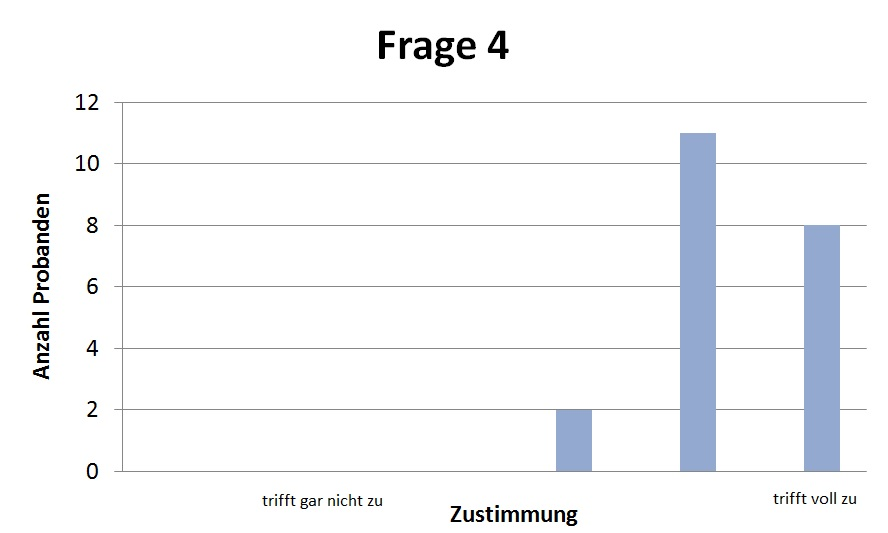
\includegraphics[width=0.7\linewidth]{img/Frage4}
\caption{Gesamtergebnis Frage 4}
\label{fig:Frage4}
\end{figure}
Diese Frage zielt auf den Gesamteindruck zum Design unseres Systems ab. Ein besonders ansprechendes Design erleichtert dem Nutzer die Bedienung, hat einen Wiedererkennungswert und bindet den Nutzer ans System. Die Ergebnisse der Evaluierung zeigen, dass die Webanwendung OfCourse bei den Testpersonen als sehr ansprechend empfunden wird.

\subsection{Frage 5}
\begin{center}
	{\it Ich könnte mir vorstellen ofCourse in einem meiner Vereine/Sportgruppen/Lerngruppen/sonstige Gruppen zu nutzen..}
\end{center}
\begin{figure}[h]
\centering
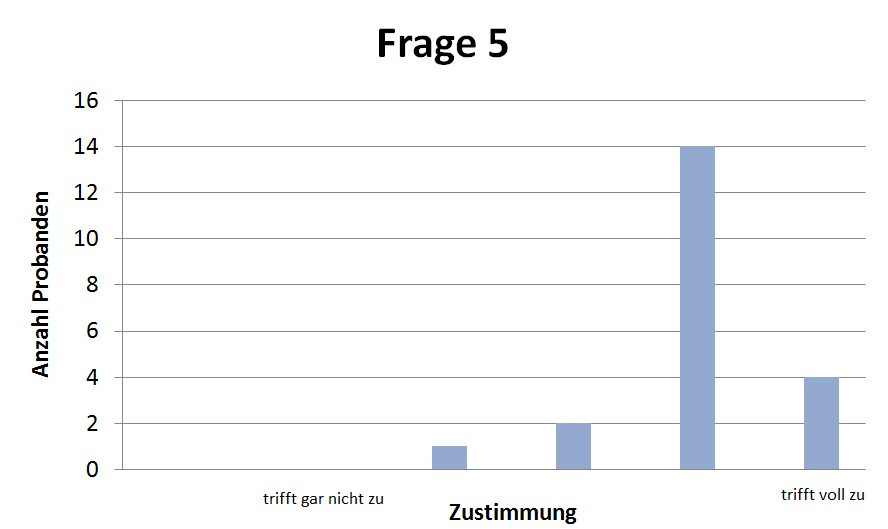
\includegraphics[width=0.7\linewidth]{img/Frage5}
\caption{Gesamtergebnis Frage 5}
\label{fig:Frage5}
\end{figure}


\subsection{Bearbeitungszeit}
Für die Bearbeitung der Tests wurde von uns eine durchschnittliche Dauer von 10 - 15 Minuten veranschlagt. Im folgenden sind die 
von den Testpersonen gebrauchten Zeiten aufgeführt.

\begin{figure}[h]
\centering
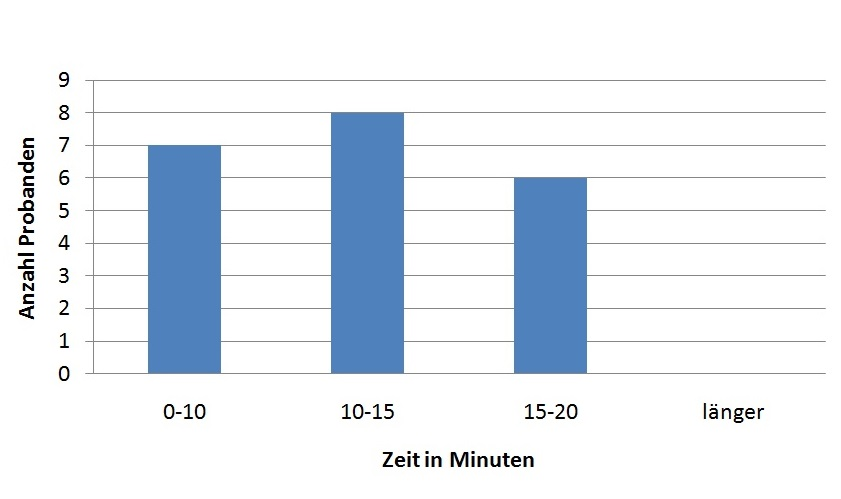
\includegraphics[width=0.7\linewidth]{img/Gesamtzeit}
\caption{Bearbeitungszeit der Tests}
\label{fig:Gesamtzeit}
\end{figure}


\subsection{Anregungen/Verbessungsvorschläge}

\section{Fazit}